% \documentclass[twocolumn, a4paper]{report}
\documentclass[a4paper]{report}

% Make section count from 1
\renewcommand\thesection{\arabic{section}}

% Custom linking
\usepackage[colorlinks = true,
            linkcolor = black,
            urlcolor  = black,
            citecolor = blue,
            anchorcolor = blue]{hyperref}
\usepackage[utf8]{inputenc}
\usepackage{booktabs}                   % For formal tables
\usepackage{url}                        % URLs
\usepackage{color}                      % For colours
\usepackage{enumitem}                   % better enumeration
\usepackage{float}                      % make graphics and tables stick
\hyphenation{Media-Eval}                % better hyphenation
\usepackage{amsmath, amssymb}           % for mathy stuff
\DeclareMathOperator*{\argmin}{arg\,min} % Jan Hlavacek

% To see subsubsecions and paragraphs in ToC
\setcounter{tocdepth}{4}
\setcounter{secnumdepth}{4}

% for \onehalfspacing and \singlespacing macros
\usepackage{setspace}
\onehalfspacing

% for quotes
\usepackage{etoolbox}
\AtBeginEnvironment{quote}{\par\singlespacing\small}

% change margin size
\usepackage[margin=3cm]{geometry}
% \usepackage[margin=2cm]{geometry}
% \setlength {\marginparwidth}{2cm}

% For graphics
\usepackage{graphicx}

% For tables
\usepackage{tabularx}
% For nice parameter descriptions (from https://tex.stackexchange.com/questions/95838/how-to-write-a-perfect-equation-parameters-description)
\newenvironment{conditions*}
  {\par\vspace{\abovedisplayskip}\noindent
   \tabularx{\columnwidth}{>{$}l<{$} @{${}={}$} >{\raggedright\arraybackslash}X}}
  {\endtabularx\par\vspace{\belowdisplayskip}}

% For page headers
% \usepackage[]{fancyhdr}

% For todos
\usepackage{xargs}                      % Use more than one optional parameter in a new commands
\usepackage[pdftex,dvipsnames]{xcolor}  % Coloured text etc.
% 
\usepackage[colorinlistoftodos, prependcaption, color=yellow]{todonotes}
\newcommandx{\unsure}[2][1=]{\todo[linecolor=red,backgroundcolor=red!25,bordercolor=red,#1]{#2}}
\newcommandx{\change}[2][1=]{\todo[linecolor=blue,backgroundcolor=blue!25,bordercolor=blue,#1]{#2}}
\newcommandx{\info}[2][1=]{\todo[linecolor=OliveGreen,backgroundcolor=OliveGreen!25,bordercolor=OliveGreen,#1]{#2}}
\newcommandx{\improvement}[2][1=]{\todo[linecolor=Plum,backgroundcolor=Plum!25,bordercolor=Plum,#1]{#2}}
\newcommandx{\rephrase}[2][1=]{\todo[linecolor=cyan,backgroundcolor=cyan!25,bordercolor=cyan,#1]{#2}}
\newcommandx{\source}[2][1=]{\todo[linecolor=Salmon,backgroundcolor=Salmon!25,bordercolor=Salmon,#1]{#2}}
\newcommandx{\definition}[2][1=]{\todo[linecolor=SeaGreen,backgroundcolor=SeaGreen!25,bordercolor=SeaGreen,#1]{#2}}
\newcommandx{\story}[2][1=]{\todo[inline, linecolor=OrangeRed,backgroundcolor=OrangeRed!25,bordercolor=OrangeRed,#1]{#2}}
\newcommandx{\conclusion}[2][1=]{\todo[inline, linecolor=Violet,backgroundcolor=Violet!25,bordercolor=Violet,#1]{#2}}
\newcommandx{\thiswillnotshow}[2][1=]{\todo[disable,#1]{#2}}
%

% To keep track of progress
\newcommand{\red}[1]{\textcolor{red}{#1}}
\newcommand{\orange}[1]{\textcolor{orange}{#1}}
\newcommand{\green}[1]{\textcolor{green}{#1}}


% For diagrams
\usepackage{adjustbox}
\usepackage{tikz}
\usetikzlibrary{fit, positioning, shapes, shapes.geometric, arrows, calc, shadows, arrows.meta}
\usepackage{subcaption}

% For code listings
\usepackage{listings}
\lstset{
  basicstyle=\ttfamily,
  columns=fullflexible,
  frame=single,
  breaklines=true,
  postbreak=\mbox{\textcolor{red}{$\hookrightarrow$}\space},
}

\usepackage{algorithm}
\usepackage{algpseudocode}
\usepackage{algorithmicx}

% Define Python style for highlighting
\lstdefinestyle{mypy}{
    language=Python,
    basicstyle=\ttfamily\small,
    commentstyle=\color{gray},
    keywordstyle=\color{blue},
    numberstyle=\tiny\color{gray},
    stringstyle=\color{red},
    showstringspaces=false,
    frame=single,
    keepspaces=true
}

% CSV
\usepackage{csvsimple}
\usepackage{longtable}
\usepackage{booktabs}

% Glossary
\usepackage[toc]{glossaries}
\usepackage[automake]{glossaries-extra}
\makeglossaries
\newglossaryentry{latex}
{
    name=latex,
    description={LaTeX (short for Lamport TeX) is a document preparation system. The user has to think about only the content to put in the document and the software will take care of the formatting}
}

\newglossaryentry{glsy}
{
    name=glossary,
    description={Acronyms and terms which are generally unknown or new to common readers}
}

\newglossaryentry{homeostasis}{
    name=Homeostasis,
    description={The regulatory process by which an organism or system maintains stability while adjusting to changing external conditions.}
}

\newglossaryentry{allostasis}{
    name=Allostasis,
    description={The process by which the body achieves stability through physiological or behavioral change in response to external or internal stressors.}
}

\newglossaryentry{operational closure}{
    name=Operational Closure,
    description={Operational closure refers to a system's operations that are functionally closed, meaning that the operations are determined by the structure of the system itself and not by its environment. In the context of cognitive systems, this means that the system's cognitive processes are primarily determined by its internal states and structures rather than direct external influences.}
}

\newglossaryentry{organizational closure}{
    name=Organizational Closure,
    description={A concept in systems theory where a system is organizationally closed if its organization is maintained over time and determines the system's interactions with its environment.}
}

\newglossaryentry{intentional stance}{
    name=Intentional Stance,
    description={A cognitive strategy to predict and explain behavior by attributing beliefs, desires, and intentions to the agent, regardless of whether the agent is a human, animal, artifact, or natural phenomenon.}
}

\newglossaryentry{grounding}{
    name=Grounding,
    description={The process of linking abstract concepts or representations to concrete experiences, perceptions, or actions.}
}

\newglossaryentry{category boundary effect}{
    name=Category Boundary Effect,
    description={A cognitive bias wherein perceivers show greater sensitivity to differences that cross a categorical boundary than to equivalent differences within a category.}
}

\newglossaryentry{poverty of the stimulus}{
    name=Poverty of the Stimulus,
    description={The argument from linguistics that children do not receive enough data from their linguistic environment to infer the complex rules of a language, suggesting an innate capability for language acquisition.}
}

\newglossaryentry{structuralism}{
    name=Structuralism,
    description={A method of interpretation and analysis of aspects of human cognition, behavior, culture, and experience that focuses on relationships of contrast between elements in a conceptual system.}
}

\newglossaryentry{post-structuralism}{
    name=Post-structuralism,
    description={A theoretical framework that critiques and extends structuralism, arguing that structures are not universally applicable and are instead specific to particular times and places.}
}

\newglossaryentry{simulation}{
    name=Simulation,
    description={The imitation of a situation or process in a model or virtual environment.}
}

\newglossaryentry{simulacrum}{
    name=Simulacrum,
    description={A representation or imitation of a person or thing, often without the substance or qualities of the original.}
}

\newglossaryentry{semiotics}{
    name=Semiotics,
    description={The study of signs and symbols and their use or interpretation.}
}

\newglossaryentry{ideomotor theory}{
    name=Ideomotor Theory,
    description={The idea that simply thinking about a movement can cause a reflexive muscular response.}
}

\newglossaryentry{agency}{
    name=Agency,
    description={The capacity of individuals to act independently and make choices or decisions.}
}

\newglossaryentry{autopoiesis}{
    name=Autopoiesis,
    description={A system's ability to reproduce and maintain itself by constantly regenerating its components in response to changes in its environment.}
}

\newglossaryentry{mary's room}{
    name=Mary's Room,
    description={A thought experiment in philosophy of mind which argues that there are non-physical properties and truths about consciousness that can't be grasped by physical facts alone.}
}

\newglossaryentry{reverse engineering}{
    name=Reverse Engineering,
    description={The process of analyzing a subject system to identify the system's components and their interrelationships, with the aim of recreating the system without copying it.}
}

\newglossaryentry{generative model}{
    name=Generative Model,
    description={In machine learning, a model that can generate new samples that are similar to, but not identical to, the training data.}
}

\newglossaryentry{constitutive autonomy}{
    name=Constitutive Autonomy,
    description={The ability of a system to maintain and modify its own organizational structure.}
}

\newglossaryentry{behavioural autonomy}{
    name=Behavioural Autonomy,
    description={The capability of a system to act in its environment based on its own internal rules and processes without external control.}
}

\newglossaryentry{fixed-action patterns}{
    name=Fixed-action Patterns,
    description={Innate behavioral responses to specific stimuli that are characteristic of a species and are often performed in a similar manner by all members of the species.}
}

\newglossaryentry{reflex-reactive-intuition-reasoning}{
    name=Reflex vs Reactive vs Intuition vs Reasoning,
    description={A classification of behavioral responses ranging from automatic reflexes, reactive responses based on learned associations, intuitive judgments that come quickly without conscious deliberation, to reasoning that involves conscious, logical thought processes.}
}

\newglossaryentry{effective action}{
    name=Effective Action,
    description={Action that brings about the desired outcome or achieves its intended purpose.}
}

\newglossaryentry{circular causality}{
    name=Circular Causality,
    description={Circular causality refers to the reciprocal and interdependent relationship between perception and action in cognitive agents, where each influences and is influenced by the other.
    }
}

\newglossaryentry{perception action cycle}{
    name=Perception-Action Cycle,
    description={}
}

\newglossaryentry{cognitive light cone}{
    name=cognitive light cone,
    description={}
}

\newglossaryentry{ontogenetic}{
    name=,
    description={scale of agent}
}

\newglossaryentry{epigenetic}{
    name=,
    description={scale of cells}
}

\newglossaryentry{phylogenetic}{
    name=,
    description={scale of species}
}

\newglossaryentry{oocyte}{
    name=,
    description={}
}

\newglossaryentry{blastoderm}{
    name=,
    description={}
}

\newglossaryentry{embryo}{
    name=,
    description={}
}

\newglossaryentry{morphospace}{
    name=,
    description={}
}

\newglossaryentry{embodiment}{
    name=,
    description={}
}

\newglossaryentry{constructivism}{
    name=,
    description={}
}

\newglossaryentry{counterfactual states}{
    name=,
    description={}
}

% \newglossaryentry{}{
%     name=,
%     description={}
% }

% \newglossaryentry{}{
%     name=,
%     description={}
% }


% \newglossaryentry{}{
%     name=,
%     description={}
% }

% \newglossaryentry{}{
%     name=,
%     description={}
% }

% \newglossaryentry{}{
%     name=,
%     description={}
% }






% Intentional Stance: The "intentional stance" is a concept introduced by the philosopher Daniel Dennett. When taking the intentional stance towards an entity (be it a human, animal, or even a machine), one interprets the behavior of the entity in terms of beliefs, desires, intentions, and other mental states. By attributing beliefs and desires to the entity, we can predict or explain its actions. Dennett contrasts this stance with two others: the "design stance" (predicting behavior based on the known purpose of the entity) and the "physical stance" (predicting behavior based on physical laws). The intentional stance is particularly useful when dealing with complex systems where the design or physical stance would be impractical.

% Functionalism: Functionalism is a philosophy of mind that proposes mental states are defined by their causal roles rather than by their physical constituents. In other words, mental states are defined by what they do and how they interact with other states and inputs/outputs, rather than what they are made of. This perspective allows for the possibility of multiple realizability, where the same mental state could be realized in different physical systems, as long as they play the same functional role.

% Computationalism: Computationalism is the hypothesis that cognition (or the mind) is a type of computation. In essence, the mind operates by processing information, akin to how a computer processes data. This perspective is often associated with the metaphor of the mind as software and the brain as hardware. It should be noted that while computationalism assumes a functional organization of the mind (in the sense that mental processes are described in terms of transformations of informational states), it is not identical to functionalism as it commits to a more specific kind of functional organization - one that is computational.

% Functional Computationalism: Functional computationalism can be seen as a specific kind of functionalism that assumes a computational perspective on the mind. It suggests that mental states are both defined by their causal roles (as per functionalism) and are computational in nature (as per computationalism). In other words, mental states are not only defined by their causal relations with other states and inputs/outputs, but these causal relations are specifically computational – they involve the transformation and manipulation of information.
%(Could be analog etc.)

% Diachronic Emergence: This term is used to describe emergent phenomena that occur over time. The term "diachronic" comes from the Greek words "dia," meaning "through," and "chronos," meaning "time." In this context, diachronic emergence refers to the idea that new properties or behaviors can emerge from a system as it evolves over time. For example, the process of natural selection leading to the evolution of new species is a form of diachronic emergence.

% Strong Asynchronic Emergence: This term is used to describe emergent phenomena that are not reducible to or predictable from the properties of their constituent parts, even in principle. The term "asynchronic" refers to the idea that these emergent properties exist at the same time as the system from which they emerge. In this context, strong asynchronic emergence refers to the idea that a system can have properties or behaviors that are fundamentally new and irreducible to the properties or behaviors of its parts. For example, consciousness might be considered a strongly asynchronically emergent property of certain complex physical systems, like brains.


% Ask GPT to add words and glossary items 


% For making fixed-width aligned columns
\usepackage{array}
\newcommand{\PreserveBackslash}[1]{\let\temp=\\#1\let\\=\temp}
\newcolumntype{C}[1]{>{\PreserveBackslash\centering}p{#1}}
\newcolumntype{R}[1]{>{\PreserveBackslash\raggedleft}p{#1}}
\newcolumntype{L}[1]{>{\PreserveBackslash\raggedright}p{#1}}

% For sidewaystable
\usepackage{rotating}


%% Defining title and subtitle
\def\thesistitle{FlowCoder}
\def\thesissubtitle{A Model of Symbolic Thought Composition via Program Synthesis using Generative Flow}


%% FOR PDF METADATA
\title{\thesistitle}
\date{\thesisdate}

\begin{document}
% \twocolumn[
%   \begin{@twocolumnfalse}
%     \begin{titlepage}
	\thispagestyle{empty}
	\newcommand{\HRule}{\rule{\linewidth}{0.5mm}}
	\center
	\textsc{\Large Radboud University Nijmegen}\\[.7cm]
	\includegraphics[width=25mm]{img/in_dei_nomine_feliciter.eps}\\[.5cm]
	\textsc{Faculty of Social Science}\\[0.5cm]
	
	\HRule \\[0.4cm]
	{ \huge \bfseries \thesistitle}\\[0.1cm]
	\textsc{\thesissubtitle}\\
	\HRule \\[.5cm]
	\textsc{\large Thesis MSc Artificial Intelligence}\\[.5cm]
	\clearpage
\end{titlepage}

%     \end{@twocolumnfalse}
%     \vspace{3cm}
%     \textbf{Student Information} \\

%     \begin{tabular}{L{3cm}l}
%                 \emph{Surname:} & \textsc{Hommelsheim} \\
%                 \emph{First name:} & \textsc{Ron} \\
%                 \emph{Student number:} & \textsc{s1000522} \\
%                 \emph{E-mail address:} & \textsc{ron.hommelsheim@ru.nl} \\
%                 \emph{Course code:} & \textsc{SOW-MKI94 (45 EC)} \\
%                 \emph{AI Specialisation:} & \textsc{Cognitive Computing} \\
%         \end{tabular}
	
%   \vspace{1cm}
%   \textbf{Supervisor Information} \\

%     \begin{tabular}{L{3cm}l}
%             \emph{Role:} & \textsc{Supervisor} \\
%             \emph{Surname:} & \textsc{Thill} \\
%             \emph{First name:} & \textsc{Serge} \\
%             \emph{Institute:} & \textsc{Radboud University} \\
%             \emph{E-mail address:} & \textsc{serge.thill@donders.ru.nl} \\
%             \emph{Supervision type:} & \textsc{Internal} \\
%     \end{tabular}
% ]







    \begin{titlepage}
	\thispagestyle{empty}
	\newcommand{\HRule}{\rule{\linewidth}{0.5mm}}
	\center
	\textsc{\Large Radboud University Nijmegen}\\[.7cm]
	\includegraphics[width=25mm]{img/in_dei_nomine_feliciter.eps}\\[.5cm]
	\textsc{Faculty of Social Science}\\[0.5cm]
	
	\HRule \\[0.4cm]
	{ \huge \bfseries \thesistitle}\\[0.1cm]
	\textsc{\thesissubtitle}\\
	\HRule \\[.5cm]
	\textsc{\large Thesis MSc Artificial Intelligence}\\[.5cm]
	\clearpage
\end{titlepage}

    \vspace{3cm}
    \textbf{Student Information} \\

    \begin{tabular}{L{3cm}l}
                \emph{Surname:} & \textsc{Hommelsheim} \\
                \emph{First name:} & \textsc{Ron} \\
                \emph{Student number:} & \textsc{s1000522} \\
                \emph{E-mail address:} & \textsc{ron.hommelsheim@ru.nl} \\
                \emph{Course code:} & \textsc{SOW-MKI94 (45 EC)} \\
                \emph{AI Specialisation:} & \textsc{Cognitive Computing} \\
        \end{tabular}
	
  \vspace{1cm}
  \textbf{Supervisor Information} \\

    \begin{tabular}{L{3cm}l}
            \emph{Role:} & \textsc{Supervisor} \\
            \emph{Surname:} & \textsc{Thill} \\
            \emph{First name:} & \textsc{Serge} \\
            \emph{Institute:} & \textsc{Radboud University} \\
            \emph{E-mail address:} & \textsc{serge.thill@donders.ru.nl} \\
            \emph{Supervision type:} & \textsc{Internal} \\
    \end{tabular}



\clearpage
\listoftodos[Notes]
\clearpage

\clearpage
\section*{Acknowledgement}
I would like to express my sincere gratitude to my supervisor for the numerous insightful discussions, indulging my every new excitement for new ideas. Their guidance and expertise have been invaluable in shaping my research and in enhancing my understanding.
Additionally, I would like to show appreciation to my parents, to my sister, and to my friends for their endless patience, encouragement, and unconditional belief in me.
Lastly, the unwavering support of my partner throughout this journey has been a constant source of motivation and inspiration, which I am greatly thankful for.

I am truly fortunate to have such a strong support network, and I am deeply appreciative of the roles each of them has played in my academic and personal development.

\begin{abstract}
    \acrfull{ai} research has historically been polarized between symbolic reasoning, characterized by precise but inflexible models, and deep learning, known for its analogical reasoning capabilities yet limited by poor generalization to \acrfull{ood} data and high data requirements. Despite the successes of \acrfullpl{llm}, challenges such as confabulation and a lack of causal reasoning persist, underscoring a gap in achieving human-like cognition. This study introduces FlowCoder, a novel program synthesizer that synergizes the symbolic and subsymbolic paradigms by embedding programs within a Transformer-based implicit world model and utilizing \acrfull{gfn} for program inference. FlowCoder demonstrates an ability in extrapolating to \acrshort{ood} tasks and performing efficient one-shot inference given sufficient training.
    This work showcases FlowCoder's capacity as a model in program synthesis and more so discusses its potential and theoretical implications as a model for a \acrfull{lot}.
\end{abstract}

\tableofcontents
\listoffigures
\listoftables

\newpage
\section{Introduction}
Imagine your brain as an interactive game engine. Just as a game engine generates dynamic virtual environments, complete with rules and physics that players interact with, the brain constructs a model of the real world. This model includes rules (physical laws, social norms), entities (objects, people), and interactions (how things work and relate to each other). We learn to navigate and predict our environment, constantly updating our internal model based on new experiences and information.
This analogy, introduced by \citet{ullmanMindGamesGame2017} extends beyond mere perception, encompassing imagination, dreams, and memory. Each of these cognitive functions can be seen as manifestations of the brain's ability to generate, manipulate, and explore various scenarios and possibilities within its internal model. Dreams and imaginative constructs, while seemingly detached from reality, are composed of the same 'material' as our waking perceptions – they are all products of the brain's simulation capabilities \cite{pearsonHumanImaginationCognitive2019}.
The self, in this view, becomes both a creator and a perceiver of its subjective reality, a reality that, while grounded in the external world, is ultimately shaped by the mind's interpretative and predictive faculties.

In the following, an overview of the fundamental concepts used in this thesis are presented, focusing on program synthesis and its relevance to understanding human cognitive processes. Strengths and limitations of current models are discussed before outlining the approach of overcoming said limitations. FlowCoder \footnote{FlowCoder is available at \url{https://github.com/R1704/master_thesis}} is introduced as a proposed model for program synthesis. A computational model and implementational details are discussed. Two experiments are outlined and their results are analyzed. Finally, improvements and various implications of the model are highlighted.

\subsection{Background}
Traditionally, \acrfull{ai} research has been approached from two general directions. \acrfull{gofai} is based on symbolic reasoning. Symbols have no internal structure but gain significance in relation to other symbols. Models based on formal reasoning are said to be precise and tend to generalize well, yet they are slow and inflexible. Instead, deep-learning relies on distributed vector representations that have a similarity structure and facilitate analogical reasoning, which may be a core function of cognition \cite{bengio2021deep,hofstadter2013surfaces}. These models tend not to generalize well to \acrfull{ood} data and are notoriously data-hungry.
Moreover, composition, systematic generalization (\acrshort{ood}), and abstraction are often argued to be crucial aspects of human cognition \cite{cholletMeasureIntelligence2019, lecun2022path,Fodor_Pylyshyn_1988, hofstadter2013surfaces, boicho2001analogical}, which may be facilitated by a latent innate capacity for the representation and construction of part-whole hierarchies 
\cite{berwickPovertyStimulusRevisited2011,fristonWorldModelLearning2021,hintonHowRepresentPartwhole2021,martinsHowChildrenPerceive2014,raussWhatBottomUpWhat2013,schwartzBehavioralNeuralConstraints2017}.

\paragraph*{Language of Thought}\label{subsubsec:pplot}
\citet{dehaeneSymbolsMentalPrograms2022} posit that human cognition is uniquely characterized by its ability to form symbolic representations and recursive mental structures akin to a \acrfull{lot}, enabling the creation of domain-specific conceptual systems. This cognitive ability allows for the generation of new concepts through the compositional arrangement of existing elements, a process exemplified by the derivation of geometric concepts \cite{alroumiMentalCompressionSpatial2021}. Cognition simplifies complex patterns into mental representations via mental compression, where the complexity of a concept is measured by the length of its mental representation as per the \acrfull{mdl} principle. 

To illustrate, when learning to play chess, rather than remembering as many games as possible, we capture the few rules, through which we can understand and explain all instances of the game.

\begin{figure}[H]
    \centering
    \includegraphics[width=0.7\textwidth]{../img/DSL.png}
    \caption{Human cognition is underpinned by multiple mental \acrfullpl{dsl}. Each language has basic building blocks - primitives which can be programmatically composed to form more complex structures. \citet{dehaeneSymbolsMentalPrograms2022} distinguish between symmetric and asymmetric programming styles. The design principles of these mental languages are shared. They are symbolic, recursive, compositional, use formal grammar, and compress programs by adhering to the minimal description length principle. The diagram was taken from the original paper \cite{dehaeneSymbolsMentalPrograms2022}.}
    \label{fig:DSL}
\end{figure}

Current versions of the \acrshort{lot} posit that the brain implements mechanisms analogous to those found in probabilistic programming languages, enabling it to represent and infer the probabilistic structure of the world \cite{lakeBuildingMachinesThat2017,ruleChildHacker2020}. A program here can be thought of a procedure that generates more examples of the same concept. If a program would represent the concept "animal", it would generate examples such as "giraffe", "zebra", "fish", and so on. Higher-level programs could produce lower-level programs. In this paradigm, the essential aspect of compositionality gives rise to a part-whole hierarchical structure, which facilitates systematic generalization.

\paragraph*{Program Synthesis and Problem Statement}
This computational model of cognition can be formalized as \emph{program synthesis}, where the goal is to automatically construct programs that satisfy a given set of specifications.
Program synthesis involves defining a domain-specific language with a set of primitives and rules, and then searching within this language for a program that satisfies a given set of input-output relations, representing the task at hand. This process is fundamentally about mapping a defined task to an executable program within the constraints of the specified \acrshort{dsl}.

A Domain-Specific Language \( \mathcal{D} \) is defined as a set of syntactic and semantic rules that determine the structure and meaning of valid expressions in the language. Formally, a \acrshort{dsl} can be represented as:
\[ \mathcal{D} = \{ \mathcal{S}, \mathcal{O}, \mathcal{R} \} \]
where \( \mathcal{S} \) is the syntax defining the structure of valid expressions, \( \mathcal{O} \) is the set of operations (or primitives) available in the language, and \( \mathcal{R} \) are the semantic rules that assign meaning to the expressions.

Primitives in the \acrshort{dsl} are the basic operations from which programs are constructed. Each primitive \( o \in \mathcal{O} \) can be thought of as a function:
\[ o: A \rightarrow B \]
where \( A \) is the set of input types and \( B \) is the output type for the primitive.

A task \( x \in X \) in program synthesis is defined as a set of input-output pairs that specify the desired behavior of a program. Formally, a task can be represented as:
\[ x = \{ (x_{in_1}, x_{out_1}), (x_{in_2}, x_{out_2}), ..., (x_{in_n}, x_{out_n}) \} \]
where each pair \( (x_{in_i}, x_{out_i}) \) consists of an input \( x_{in_i} \) and the corresponding desired output \( x_{out_i} \).
The objective of program synthesis is to find a program \( \rho \) within the language \( \mathcal{D} \) that satisfies the task \( x \). Formally, this can be seen as a search problem:
Find \( \rho \in \mathcal{D} \) such that for every \( (x_{in_i}, x_{out_i}) \in x \), \( \rho(x_{in_i}) = x_{out_i} \).

\paragraph*{DreamCoder}\label{subsubsec:dreamcoder}
\acrfull{dc} stands out as a particularly effective model in program synthesis, creating programs from basic primitives and tasks with the goal of developing its own domain-specific language \cite{ellisDreamCoderBootstrappingInductive2021}. It employs an adapted wake-sleep algorithm, initially introduced by \citet{hinton1995wake}, to simultaneously train a generative model and a recognition network. The generative model is tasked with learning a probability distribution across programs, while the recognition network is designed to map tasks to specific programs, facilitating a neurally-guided exploration of the program space. This process leverages the recognition network to implement a parallel search strategy, blending best-first and depth-first searches to prioritize programs based on their probabilities.

The model significantly narrows the search scope by abstracting frequently used sub-routines into more readily accessible concepts, thereby enhancing scalability. This abstraction not only reduces the depth of the search tree but also limits its breadth, with the abstraction phase playing a pivotal role in refactoring subroutines in accordance with the \acrlong{mdl} principle and in the learning of the \acrlong{dsl}.

The tasks addressed by DreamCoder can either be generative, such as image creation, or conditional, like establishing input-output relationships for list sorting. Examples of tasks from various domains are depicted in \autoref{fig:conc_library}(A), while \autoref{fig:conc_library}(B) illustrates the process of learning to sort a list. The figure shows initial primitives on the left, a middle section highlighting the library of learned concepts and the established part-whole hierarchy, and on the right, the ultimate solution employing \texttt{concept15}, which itself incorporates previously abstracted concepts.

\begin{figure}[H]
    \centering
    \includegraphics[width=\textwidth]{../img/conc_library.png}
    \caption{(A) Tasks across eight distinct domains. (B) Illustration of the concept library that has been acquired. The left side displays the foundational primitives that are used to construct the concepts shown in the central area. To the right, a task is presented through input-output relationships alongside the derived solution. Below, this solution is reformulated using solely the initial primitives. Image taken with permission from the original paper \cite{ellisDreamCoderBootstrappingInductive2021}.}
    \label{fig:conc_library}
\end{figure}


\paragraph*{DeepSynth}

\citet{fijalkowScalingNeuralProgram2021} propose a framework called "distribution-based search", in which they investigate the difficult problem of searching through a \acrshort{dsl} to find programs matching a specification in a vast hypothesis space.
They introduce DeepSynth \footnote{\url{https://github.com/nathanael-fijalkow/DeepSynth}}, a general-purpose program synthesizer which constructs programs from input-output examples, and a useful framework allowing us to test different models and search methods, which I am using in this project.
The authors discuss different program finding strategies. Specifically, they find that both enumerative search (as in \acrshort{dc}) and sampling are viable strategies, where search is associated with prioritizing quantity, i.e. creating many programs quickly, whereas sampling strategies prioritize quality but may be slower, since resampling may occur. An additional benefit of sampling over search is space efficiency - already created programs don't need to be memorized.
Here, an initial \acrshort{dsl} along with suitable syntactic constraints compile into a \acrfull{cfg}, defining the possible structures of programs within its \acrshort{dsl}. A \acrshort{cfg} consists of a set of production rules that describe how to generate strings from a set of non-terminal and terminal symbols. It is "context-free" because the production rules are applied regardless of the surrounding symbols.
In DeepSynth, a prediction model is used to predict weights for a \acrfull{pcfg}, extending the \acrshort{cfg} by associating probabilities with the production rules. This allows the grammar to not only generate the syntactic structure of a program but also to represent beliefs about the relative plausibility or frequency of different structures \footnote{See appendix \autoref{app:cfg} for a formalization of \acrshortpl{cfg} and \acrshortpl{pcfg}.}. This is similar to DreamCoder's prior, consisting of a library of sub-routines combined with a weight vector. The \acrshort{pcfg} guides the search and inference process towards more likely programs. DreamCoder however, does not specifically use a \acrshort{pcfg}. Both frameworks employ a typed $\lambda$-calculus, hence there are restrictions on program arguments, etc. (syntactical constraints). DreamCoder performs type inference during program generation. To spare computational cost, DeepSynth constructs the \acrshort{cfg} beforehand which in turn increases its size.
\citet{fijalkowScalingNeuralProgram2021} compare different search strategies and show that methods that do not use a machine-learned \acrshort{pcfg} (e.g. \acrfull{dfs}) barely solve any tasks, demonstrating the necessity for better strategies.

\subsection{Limitations}
Although DreamCoder and DeepSynth prove to be successful in synthesizing programs, their methods reveal a foundational limitation: their heavy reliance on syntactical constraints.
While these constraints are undoubtedly vital for ensuring the correctness of generated programs, they do not necessarily guarantee a deep understanding or utilization of semantic relationships within the code. Additionally, \citet{kimCompoundProbabilisticContextFree2019} explain that associating only a scalar per rule misses a lot of information. A distributed representation of the \acrshort{dsl} would therefore be beneficial. We could imagine a program space in which certain symmetries could be leveraged. One could argue e.g. that "\(+\)" is to "\(-\)" as "\(\div\)" is to "\(\times\)". These semantic relationships may be missed in the previously discussed models.

\subsection{Approach}
\paragraph*{Transformers and Self-Attention}
The Transformer architecture, originally introduced in 2017 by \citet{vaswaniAttentionAllYou2017}, has proved to be widely successful in a wide range of applications \cite{wolfTransformersStateoftheArtNatural2020,khanTransformersVisionSurvey2022}. Transformers use self-attention, a mechanism that enables dynamic selection and focus on specific parts of the input, as opposed to treating all parts equally. It effectively allows the network to "attend" to, or give more weight to, certain inputs over others during the processing stage. The self-attention mechanism allows for an understanding of not just the structural arrangement of elements in a sequence (syntax) but also their deeper, contextual relationships (semantics) \cite{wolfram2023chatgpt}. In this thesis I will use this model for a rich representation of programs. However, training the Transformer is difficult from only a few examples. Therefore, I will combine the approach with an amortized sampler, explained in the following.

\paragraph*{GFlowNet}
\acrfullpl{gfn}, introduced by \citet{bengioFlowNetworkBased2021}, are a class of generative models designed to learn to construct compositional objects from a target distribution over complex high-dimensional spaces, particularly where explicit density estimation is challenging and diverse candidates are encouraged. \acrshortpl{gfn} learn a stochastic policy for generating sequences of actions that lead to the construction of a sample. The model generates sequences of actions that build a sample, with the generation frequency of each sample being proportional to an associated reward function.
In other words, \acrshortpl{gfn} are applicable in problems where complex structures are composed from simple building blocks and have been used in molecular composition from atoms \cite{bengioFlowNetworkBased2021}, in grammar induction \cite{Hu_Malkin_Jain_Everett_Graikos_Bengio_2023}, and in Bayesian structure learning \cite{deleuBayesianStructureLearning2022}. The learnt policy becomes an amortized sampler. This means that the extensive training invested in the model results in a system capable of efficiently generating new samples without the need for additional, extensive computation for each new instance. Moreover, the model can be used for offline training, i.e. from data that is not from the observed distribution. This aspect is crucial for \acrshort{ood} generalization and may be the remedy for data-hungry Transformers.

\subsection{Research Question, Aim, Motivation}
In recent advancements, \acrfull{sota} models like \acrlong{dc} have demonstrated proficiency in program synthesis. However, they often lack a semantically rich state representation and heavily rely on search algorithms for constructing programs. This thesis aims to investigate a novel approach by combining the strengths of two distinct architectures: the Transformer and \acrshort{gfn}. The Transformer architecture is known for its ability to learn rich state spaces, albeit with a significant data requirement and limited generalization to \acrlong{ood} tasks. On the other hand, \acrshort{gfn}, with its capability for amortized sampling, presents a promising solution to overcome these challenges. The central hypothesis of this thesis is that the integration of these two architectures could yield a powerful program synthesizer. This synthesizer would be capable of solving tasks with minimal examples, specifically in the list-editing domain. 
Furthermore, theoretical and computational challenges are identified and addressed within the realm of neural program synthesis.

This research explores the potential alignment of the proposed model with the \acrlong{lot} hypothesis, suggesting a programming language-like mental representation underpinning human thought. 
Thus, this research not only aims to address a practical gap in program synthesis but to explore the role of program synthesis in a model of cognition, thereby contributing to the philosophical and psychological understanding of thought, and intelligence. 

\subsection{Scope and Limitations}
The concept of abstraction in program synthesis is necessary for the model to learn its own \acrshort{dsl}. Abstraction effectively narrows the depth of the search tree through program refactoring and identifies common patterns, thereby aiding in generalization. Additionally, abstraction is essential in optimizing for the \acrlong{mdl}, which is a useful inductive bias humans seem to employ \cite{sable-meyerLanguageThoughtMental2022}.
However, in this research, abstraction was not implemented. This decision was primarily guided by time constraints. As a result, I focus on modeling a program synthesizer that solves tasks and on testing its abilities, rather than additionally learning the \acrshort{dsl}. Consequently, it is anticipated that the model will not optimize for parsimonious programs.


% \subsection{\red{Main Contributions}}
% FlowCoder \footnote{Code available at \url{https://github.com/R1704/master_thesis}}.
% % Highlight the significance of your research within the field of AI. Explain how your work contributes to advancing knowledge or addressing the identified research gap. Mention the potential impact of your findings or proposed solutions.
% % The main contributions of this thesis are: 
% % \begin{itemize}
% %     \item I argue that the same multi-scale hierarchies that govern biological organization can be applied to the conceptual realm
% %     \item I develop a method of bayesian program synthesis, using GFlowNet
% %     \item I present the philosophical ramifications
% % \end{itemize}

% % \begin{itemize}
% %     \item novel program synthesizer FlowCoder
% %     \item philosophical ramifications as a model of cognition
% %     \item results 
% %     \item conclusion.
% % \end{itemize}





% I present a novel method for program synthesis and show that systematic generalization is achievable without explicit world models, i.e. without parameterizing a \acrshort{dsl} or \acrshort{pcfg}. Rather, implicit world models in the form of Transformers may be sufficient. I discuss the consequences of the two variants and propose extensions to my model. 

\newpage
\section{Methods}
In the following, the foundational concepts used within this thesis are outlined in detail. The proposed model, FlowCoder, is introduced and an exact computational model is given, before describing implementational details and training and testing strategies.
\subsection{Foundations \& Computational Framework}

\paragraph*{\acrshort{gfn}} \acrshortpl{gfn} create a \acrfull{dag} over the state space, where vertices correspond to states or partial samples and edges denote transitions or adding a component to a partial sample, in which the edges carry a flow from source to targets \cite{bengioFlowNetworkBased2021}.
In \acrshortpl{gfn}, the "flow" in the network corresponds to the process by which the network constructs a sample, which can be thought of as a path in a graph where nodes are partial samples, and edges correspond to adding a component to the partial sample.
The core training objective for a \acrshort{gfn} is to satisfy the flow matching constraint. The idea is to ensure that the flow into any state (a partially constructed sample) matches the flow out of it, given the reward associated with complete samples. The flow here refers to the expected transitions into or out of a state under the model's stochastic policy. 

Formally, a state \( s \) represents a partial object a certain stage in the generative process. A trajectory \( \tau \) is a sequence of states \( s_0, s_1, ..., s_T \); the model traverses from an initial state \( s_0 \) to a terminal state \( s_T \), where the target structure is complete.
A trajectory \( \tau \) is formed by a sequence of actions \( a_1, a_2, ..., a_T \), where each action \( a_t \) transitions the model from state \( s_{t} \) to state \( s_{t+1} \). The sequence of actions is governed by a policy \( \pi \), which defines the probability of choosing a particular action given the current state.
The flow \( F(\tau) \) of a trajectory \( \tau \) is defined as the product of the probabilities of each transition along the trajectory, multiplied by the reward \( R(s_T) \) of the terminal state, normalized by a partition function \( Z \).

\begin{equation} \label{eq:flow}
    F(\tau) = \frac{R(s_T)}{Z} \prod_{t=0}^{T-1} \pi_\phi(s_{t+1} | s_{t})
\end{equation}

The partition function \( Z \) ensures that the sum of flows over all possible trajectories equals one, effectively normalizing the distribution. Since we don't know \( Z \), we can estimate it by parameterizing it as \( Z_{\theta} \).
The flow matching constraint enforces that for any given non-terminal state \( s \), the total flow into \( s \) must equal the total flow out of \( s \):

\begin{equation} \label{eq:flow_match}
    F(\tau) = F(\tau')
\end{equation}

where \( F(\tau') \) is the reverse trajectory. The partition function is estimated and utilized to balance the probabilities throughout the \acrshort{dag}.
Following \citet{malkinTrajectoryBalanceImproved2022}, we can utilize this property to create a suitable loss function - \acrfull{tb} Loss to train the \acrshort{gfn}. 

\begin{equation}\label{form:TB}
    \mathcal{L}_{TB} = \left(\log Z_\theta(x) + \sum_{t=0}^{T-1} \log \pi_\phi(s_{t+1}|s_{t}, x) - \log R(s_T \vert x)\right)^2
\end{equation}     

Here $s_T$ is a constructed object, in this case a program $\rho$. The complete derivation of the TB loss can be found in \autoref{app:TB}. \\
To compute the reward $R(\rho | x)$, the sampled program $\rho$ is executed and evaluated to get $\rho(x_{in}) = \tilde{x}_{\text{out}}$ after which the output pair $(x_{\text{out}}, \tilde{x}_{\text{out}})$ is compared. \\
Additionally, a state-task representation is encoded by $T_\theta(x, s_t)$, parameterized by $\theta$. In this project, $T$ will be referred to as state-task representation or generative model interchangeably. The output $z = T_\theta(x, s_t)$ is the task-state representation which policy $\pi$ takes as an input.

\paragraph*{\acrfull{em}} \acrlong{em} is an algorithm for finding maximum likelihood estimates in models with latent variables. It iteratively optimizes a lower bound on the likelihood of the observed data, alternating between inferring the most likely latent states (E-step) and optimizing model parameters given these states (M-step) \cite{han2022data}. \acrshort{em} has been used repeatedly in in the realms of grammar induction or program synthesis. DreamCoder uses a generalized version of \acrshort{em} \cite{ellisDreamCoderBootstrappingInductive2021}. \citet{kimCompoundProbabilisticContextFree2019} use \acrshort{em} for grammar induction and \citet{Hu_Malkin_Jain_Everett_Graikos_Bengio_2023} extend \citeauthor{kimCompoundProbabilisticContextFree2019}'s \cite{kimCompoundProbabilisticContextFree2019} methodology, and propose a novel method GFlowNet-EM. Similar to \citet{Hu_Malkin_Jain_Everett_Graikos_Bengio_2023}, I am updating the two models separately.

In the E-step a program $\rho$ is sampled and the parameters of policy $\pi_\phi$ are updated using the Trajectory Balance Loss (\autoref{form:TB}). Here, the policy tries to find better programs solving the task. \\
The M-step comprises sampling a program $\rho$ and updating the model parameters $T_\theta$ with reward $-\log R(\rho|x)$, where the goal is to refine the generative model.

\paragraph*{Sleep} Inspired by DreamCoder and GFlowNet-EM, I am employing a modified wake/sleep algorithm, originally introduced by Hinton et al. \cite{hinton1995wake}. 

In \emph{Replay}, the forward policy is trained on previously solved task-program pairs $(x, \rho)$, using the trajectory $\tau$ to guide the model to the correct solution and optimizing on the forward logits. Here $x$ is sampled from the empirical distribution and $\rho$ is sampled from the forward policy $\pi_\phi$. Additionally, a sleep weight $\gamma$ is applied to strengthen the gradient. Formally:
\begin{equation}
    \nabla_\phi\mathcal{L}_{\text{Replay}} = \mathbb{E}_{x \sim X, \rho \sim \pi_\phi(\centerdot|x)} \left[ - \gamma \cdot \log \pi_\phi(\tau \vert x, \rho) \right]
\end{equation}
If a correct solution has been found during the E-step, I immediately let the model train on these trajectories of correct solutions so as to consolidate these.
After the E-step I again train the model on a set (in the mathematical sense, meaning no duplicates) of all the correct solutions, so that it doesn't forget solutions to other tasks.
Replay is applied stochastically, given the hyperparameter $\xi$.
    
During \emph{Fantasy}, the policy is trained on hypothesized programs with tasks from the empirical distribution. Programs are executed using task \emph{inputs} from the empirical distribution to output a predicted \emph{output} and thus create correct task-program pairs $(\tilde{x}, \rho)$. Programs that produce unwanted behavior such as producing constants (that are not dependent on the task), or NaNs are filtered out. Then, similarly to the methodology of Replay, the model is trained on these pairs. Formally:
    \begin{equation}
        \nabla_\phi\mathcal{L}_{\text{Fantasy}} = \mathbb{E}_{x \sim X, \tau \sim \pi_\phi(\centerdot|x)} \left[ - \gamma \cdot \log \pi_\phi(\tau \vert \tilde{x}, \rho) \right]
    \end{equation}
Fantasy is also applied stochastically, given the hyperparameter $\sigma$. 
Incorrectly proposed programs or randomly generated programs allows the model to learn which task-program pairs do or do not make sense, while fantasy on correct programs allows the model to generalize programs to different input-output pairs.

\paragraph*{Optimization Techniques} \citet{Hu_Malkin_Jain_Everett_Graikos_Bengio_2023} propose several optimization techniques that I adopted in this project. These will be described in the following.
\begin{description}
    \item[E-step Loss Thresholding] Rather than training the GFlowNet to a loss of zero after each M-step, we can apply a linearly decreasing moving average loss $\delta$ as a threshold to trigger the M-step using the hyperparameter $\alpha$, to save computational cost. Here I use the recursive formula:
    \begin{equation}\label{eq:threshold}
        \delta = \alpha \cdot \mathcal{L}_{TB} + (1 - \alpha) \cdot \delta
    \end{equation}
    \item[Exploration] Since we want to find many modes in the E-step and want to avoid getting stuck in local optima, several exploration techniques can be employed.
    The hyperparameter $\{\beta \vert \beta \in \mathbb{R}_{[0, 1]} \}$ can be used to exponentiate the forward policy: $ \pi_\theta(s_{t+1}|s_t)^\beta $.
    Moreover, $\epsilon$-uniform sampling can be used to the deter the model from repeating known routes by mixing the predicted logits with a uniform distribution. $\epsilon$ is chosen to be $\{\epsilon \vert \epsilon \in \mathbb{R}_{[0, 1]} \}$.
\end{description}

\subsection{FlowCoder}

\paragraph*{Program Representation} DeepSynth represents programs as \acrfullpl{ast}. An \acrshort{ast} is a tree representation of the syntactic structure of the program, with nodes representing operations or primitives and edges representing their compositional relationships. Other common methods in program synthesis are used such as deBruijn indexing, which is a technique to represent bound variables in a way that avoids naming conflicts and simplifies variable substitution \cite{debruijnLambdaCalculusNotation1972}. Named variables are replaced with numeric indices representing the number of enclosing $\lambda$-abstractions that bind the variable. See \autoref{fig:AST} for a visualization of an \acrshort{ast}. Moreover, the authors implement a polymorphic type system which facilitates the constraint of compiling a \acrshort{cfg} that produces programs of a desired type-request \footnote{The DeepSynth implementation can be found at \url{https://github.com/nathanael-fijalkow/DeepSynth}}.

\begin{figure}[H]
    \centering
    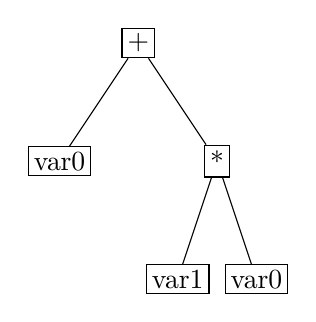
\begin{tikzpicture}
        [
        every node/.style={draw, inner sep=2pt},
        level distance=1.5cm,
        level 1/.style={sibling distance=2cm},
        level 2/.style={sibling distance=1cm}
        ]
        
        \node {+}
        child {
            node {var0}
        }
        child {
            node {*}
            child {
            node {var1}
            }
            child {
            node {var0}
            }
        };
    \end{tikzpicture}
    \caption{An example of an abstract syntax tree (AST). This translates to the function \texttt{f = var0 + var1 * var0}.}
    \label{fig:AST}
\end{figure}








% \begin{figure}[H]
%     \centering
%     \begin{tikzpicture}
%         [
%         every node/.style={draw, inner sep=2pt},
%         level distance=1.5cm,
%         level 1/.style={sibling distance=2cm},
%         level 2/.style={sibling distance=1cm}
%         ]
        
%         \node {map}
%         child {
%             node {var0}
%         }
%         child {
%             node {*}
%             child {
%             node {var1}
%             }
%             child {
%             node {var0}
%             }
%         };
%     \end{tikzpicture}
%     \caption{An example of an abstract syntax tree (AST). This translates to the function \texttt{f = var0 + var1 * var0}.}
%     \label{fig:AST}
% \end{figure}





% All modules are written using PyTorch \cite{NEURIPS2019_9015}.





\paragraph*{Generative Model}\label{sec:gen_model}
To embed programs effectively within a neural network, it is essential to represent them in a format that is compatible with the neural network's architecture. Abstract syntax trees, which are inherently 2-dimensional and include information of parent, children and sibling nodes, should be translated into a neural network format while ensuring the preservation of this valuable structural information.
Various concepts have emerged, including using \acrfullpl{gnn}, see e.g. \cite{allamanis_learning_2018,velickovicCLRSAlgorithmicReasoning2022,bieber_learning_2020,ibarz_generalist_2022}. Others proposed special Tree-Transformers which are able to encode \acrshortpl{ast}, see e.g. \cite{pengRethinkingPositionalEncoding2022,wang2017dynamic}.
\citet{heTreesTransformersTheoretical2021} find that standard Transformers achieve similar results to Transformers where tree position information is explicitly encoded. This is presumably because of the positional encoding, which is a way of adding fixed sinusoidal functions with different frequencies and phases to the embeddings of tokens in a sequence, enabling the neural network to discern the position of each tokens through these distinctive patterns; and more importantly, because of the fundamental component of the Transformer, which is the self-attention mechanism, formalized as \cite{vaswaniAttentionAllYou2017}:
\begin{equation}
    \text{Attention}(Q, K, V) = \text{softmax}(\frac{QK^T}{\sqrt{d_k}})V
\end{equation}

This mechanism, through the query (Q), key (K), and value (V) matrices, allows the model to dynamically assign importance to different parts of the input sequence. The scaling factor $\sqrt{d_k}$ normalizes the dot product, aiding in stabilizing gradients during training. Moreover, the Transformer employs Multi-Head Attention, enabling the model to concurrently process information from different representation subspaces, enhancing its capability to capture diverse features. 
Therefore, I decided to use the standard Transformer architecture, which takes a 1-dimensional sequence as an input, meaning the \acrshort{ast} has to be linearized. 

Rather than embedding the primitives of the DSL to construct \acrshortpl{ast}, the already preprocessed rules of the context-free grammar are embedded, created in conjunction with the syntactic constraints, thus essentially predicting edges rather than nodes. The array of \acrshort{cfg} rules has to be converted back to \acrshort{ast} format for evaluation, which can be easily done within the DeepSynth framework.
In a plausible model of cognition, we don't possess an explicit representation of the \acrshort{cfg} but rather infer it.
However, in the case of DeepSynth, it generates a more extensive \acrshort{cfg} instead of conducting type inference, which is the approach employed in DreamCoder. Consequently, a lookup to identify the syntactically permitted rules must be performed, thereby filtering out those that do not conform to the syntax. Naturally, in principle the model could be allowed to generate syntactically incorrect programs and assign them a reward of 0 during evaluation, but to expedite the learning process, I refrain from doing so.

\begin{description}
    \item[The RuleEncoder] begins by collecting rules, which are pairs of non-terminals and corresponding program actions, from the \acrshort{cfg} and adds special tokens such as 'PAD' (padding), 'START' (sequence start), and 'STOP' (sequence end). Each rule is passed through an embedding layer.
    During the forward pass, batches of state sequences (each state sequence, or trajectory $\tau$, representing a series of \acrshort{cfg} rules) are processed. To ensure uniformity across different sequences within a batch, padding is applied.
    \item[The IOEncoder] is tasked with encoding \acrfull{io} pairs into continuous vector representations.
    Each input-output pair is tokenized using a predefined lexicon (a list of symbols representing the possible range of inputs and outputs), which includes special tokens such as 'PAD' (padding), 'IN' (input start), and 'OUT' (output start). This tokenization is critical for distinguishing between different parts of the input-output pairs.
    The tokenized input-output pairs are concatenated into a single sequence, with the 'IN' and 'OUT' tokens demarcating the transition from input to output. Padding is then applied to ensure that all sequences have the same length, aligning them to the maximum allowed size determined by \texttt{n\_examples\_max} (the maximum number of input examples that can be processed) and \texttt{size\_max} (the maximum size of elements in a list). These parameters have been adapted from DeepSynth. The padded sequences are passed through an embedding layer. This embedding is crucial for capturing the semantic relationships between different tokens.
    \item[The Transformer] initializes with the IOEncoder and the RuleEncoder. Positional Encoding is applied to the output of both encoders. This step is vital as it adds information about the sequence order to the model, allowing the Transformer to interpret the sequence data effectively.
    The Transformer employs two types of masks: padding masks for IO sequences and square subsequent masks for state sequences. The padding mask ensures that the model does not process padding tokens, while the square subsequent mask prevents positions from attending to subsequent positions, maintaining the autoregressive property in the generation process.
\end{description}

\paragraph*{Forward Policy}
At each step, the forward policy takes the Transformer output as an encoded state and predicts log probabilities over the \acrshort{cfg} rules, after which softmax is applied to get a distribution between 0 and 1 and sample the next action. 
The forward policy is implemented as a \acrfull{mlp} and predicts forward logits from the Transformer's output, guiding the generative process.

\paragraph*{Partition Function}
The partition function $Z_\theta$, which is an estimation of the sum of all rewards $R(\rho|x)$, serves as a normalizing factor, ensuring that the probabilities generated by the model are well-calibrated and interpretable. It is implemented as a \acrshort{mlp} layered on top of the Transformer, outputting a scalar.

See \autoref{table:params} for the exact parameterization of the models.

\paragraph*{Sampling Programs}\label{sec:sampling_programs}
In the process of constructing an Abstract Syntax Tree, there exists flexibility in the order of expansion. Nodes can be expanded in a depth-first, breadth-first, etc. manner, or for instance, one can adopt a bottom-up approach, wherein terminal nodes are predicted initially and subsequently connected in a progressive manner. This approach offers the advantage of enabling the evaluation of partial expressions, which, in turn, can serve to inform the model and enhance computational efficiency, albeit at the expense of increased memory requirements. Alternatively, we may consider employing a model akin to the forward policy, predicting the subsequent node (or edge) to be expanded.
However, I chose to sample the actions for the tree construction in a depth-first manner, mainly for two reasons. 
First, for simplicity, and second so that the AST when linearized always has the same order, potentially giving the Transformer a useful inductive bias.

Specifically, the state of each program in the batch is initialized with a 'START' token, representing the initial state of the program generation process. A frontier, implemented as a queue, is initialized for each program to manage the sequence of non-terminals that need to be expanded. This method has been adapted from DeepSynth to fit with the FlowCoder framework and mechanisms. 
The core of the method is a loop that continues until all frontiers are empty, indicating that all programs in the batch have been fully generated. Within this loop, the model computes logits and partition functions.
The sampling method includes an exploration mechanism, where with a probability $\epsilon$, uniform sampling is used instead of the model's logits. This exploration is crucial for introducing variability and avoiding local optima in the generation process. Additionally, tempering is applied to logits using a factor $\beta$, modulating the sharpness of the probability distribution used for sampling.
For each program in the batch, the method iteratively samples a rule based on the current non-terminal and updates the program's state and cumulative logits. This process involves creating a mask to block invalid actions, applying the mask to logits, and sampling an action (rule) based on the masked logits.
Each sampled rule is decomposed into a non-terminal and program component, updating the program's current state and expanding the frontier with the rule's arguments.
Once all frontiers are empty, the final programs are reconstructed from their compressed representations, using methods provided by DeepSynth.

\paragraph*{Reward} \label{sec:reward}
In order to train the model, a reward function has to be operationalized. Various approaches exist for this purpose, the simplest being a binary reward, as employed in DreamCoder. Does the output of the program match the actual output or not? A binary reward however, is not very informative. A reward that provides a gradient is much more useful. \citet{bengioGFlowNetFoundations2023} propose an \acrfull{ebm}, wherein the model learns to associate favorable outcomes with low energy states and unfavorable outcomes with high energy states. I found that this method introduced unnecessary complexity to the model. Instead, the Levenshtein edit distance was used \footnote{The implementation of the Levenshtein distance I used can be found at \url{https://github.com/maxbachmann/Levenshtein}}, which is a measure of the similarity between two strings \cite{Levenshtein}. Specifically, it quantifies the minimum number of single-character edits (i.e., insertions, deletions, or substitutions) required to transform one string into another. See the appendix (\autoref{app:levenshtein}) for an in depth formalization of the metric.
Since the Levenshtein distance returns a discrete value, it was normalized over the maximum length of the sequences, and since there may be more than one example per task, it was averaged over all examples. Moreover, a maximum reward parameter was applied, to scale a correct solution up and give the model a stronger gradient. In my experiments a maximum reward of 10 was used.


\subsection{Design} \label{subsec:design}
In the following section I will elaborate on the exact training and test methods employed, including hyperparameters.
The tasks that were used are input-output relations in the list editing domain, originally from DreamCoder, see \autoref{tab:task_ex} for examples. These were filtered given the syntactic constraints (e.g. type, lexicon, etc.) and provided by DeepSynth. 
In their paper, \citet{fijalkowScalingNeuralProgram2021} discuss that some of the tasks are impossible to solve given the DSL, therefore, those were additionally filtered out, finally leaving 95 tasks in the dataset. Tasks can be of a similar variety (e.g. \texttt{add-k with k=1} and \texttt{add-k with k=2} belong to the same group). There are 25 such task groups in total. Each task can have between 1 and 15 examples. A task is considered solved if a program solves all examples of the task \footnote{All tasks can be found in my GitHub repository.}.
The DSL is essentially a dictionary of primitive types and semantics in a typed $\lambda$-calculus, including functions like \texttt{index}, \texttt{car}, \texttt{append} as well as numerical functions like \texttt{+}, \texttt{*}, \texttt{mod}, \texttt{is-prime}, etc., all written in Python (\autoref{app:dsl}).
\autoref{tab:synconst} describes the syntactical constraints used in the experiment, which were mostly adapted from DeepSynth and DreamCoder.

\begin{table}[H]
    \centering
    \begin{tabularx}{\textwidth}{|l|l|X|}
        \hline
        \textbf{Parameter} & \textbf{Value} & \textbf{Description} \\\hline
        \texttt{type} & \texttt{list(int) $\rightarrow$ list(int)} & The input as well as the output should be a list of integers, so the CFG should reflect that, filtering rules that do not conform to that criterion. \\\hline
        \texttt{lexicon} &  $[-30, 30] \in \mathbb{Z}$ & The lexicon is a uniform distribution of integers and in the range from -30 to 30 \\\hline
        \texttt{maximum argument number} & 1 & This is the maximum number of arguments a function could have. \\\hline
        \texttt{size max} & 10 & The maximum number of values in a list \\\hline 
        \texttt{max number of examples} & 15 & The maximum number of examples per task \\\hline 
    \end{tabularx}
    \caption{Syntactical Constraints}
    \label{tab:synconst}
\end{table}

All experiments were trained in random order with a batch size of 4 where each task in the batch is the same. This was done to avoid a credit assignment problem while increasing efficiency. Since the forward logits are summed up and averaged over for all trajectories, training the model at multiple task at once might have confused which trajectory was rewarding. However, batching, especially when training on a GPU has computational benefits.
Furthermore, each task is trained for 5 epochs with 2.000 E-steps and 2.000 M-steps in each epoch. The moving average threshold (see \autoref{eq:threshold}) $\delta$ was initialized with 150 and linearly decreases using the hyperparameter $\alpha$ set to $0.3$. The exploration parameters $\beta$ and $\epsilon$ were set to $0.7$ and $0.3$, respectively. The sleep weight $\gamma$ was set to 10 on all experiments. 
The learning rates for the generative model as well as for the forward policy were set to $0.0001$. During inference I ran the model for $100$ steps. Since the batch size is 4, this creates 400 programs per task. A table of all hyperparameters can be found in \autoref{app:hyperparams}. The experiments were run on a single NVIDIA Tesla T4 GPU. Throughout the five epochs, each consisting of 2.000 E- and M-steps with a batch size of four, the model generated approximately 80.000 programs per task.

\begin{table}[ht]
    \centering
    \begin{tabular}{|p{5cm}|c|c|}
        \hline
        \textbf{Task} & \textbf{Input} & \textbf{Output} \\\hline
        \texttt{remove gt 2} & \texttt{[1,2,7,5,1]} & \texttt{[1,2,1]} \\\hline
        \texttt{caesar-cipher-k-modulo-n with k=5 and n=4} & \texttt{[2, 2, 0, 1, 2, 3, 3]} & \texttt{[3, 3, 1, 2, 3, 0, 0]} \\\hline
        \texttt{prepend-index-k with k=3} & \texttt{[15, 12, 9, 14, 7, 9]} & \texttt{[9, 15, 12, 9, 14, 7, 9]} \\\hline
        \texttt{add-k with k=4} & \texttt{[16, 10, 7, 12, 13, 3]} & \texttt{[20, 14, 11, 16, 17, 7]} \\\hline
        \texttt{append-k with k=2} & \texttt{[1, 5, 15]} & \texttt{[1, 5, 15, 2]} \\\hline
    \end{tabular}
    \caption{Task Examples}
    \label{tab:task_ex}
\end{table}


\begin{table}[ht]
    \centering
    \begin{tabular}{|p{5cm}|c|}
        \hline
        \textbf{Task} & \textbf{Program} \\\hline
        \texttt{remove gt 2} & \texttt{(filter (gt? 3) var0)} \\\hline
        \texttt{caesar-cipher-k-modulo-n with k=5 and n=4} & \texttt{(map (mod 4) (map (+ 5) var0))} \\\hline
        \texttt{prepend-index-k with k=3} & \texttt{(cons (index 2 var0) var0)} \\\hline
        \texttt{add-k with k=4} & \texttt{(map (+ 4) var0)} \\\hline
        \texttt{append-k with k=2} & \texttt{(append 2 var0)} \\\hline
    \end{tabular}
    \caption{Examples of tasks and programs solving the tasks.}
    \label{tab:task_programs}
\end{table}


























% The full algorithm is described in the pseudocode: \autoref{alg:flowcoder}. 



% \begin{algorithm}[H]
%     \caption{FlowCoder}
%     \begin{algorithmic}[1]
%     \Require Data $X$, generative model with parameters $\theta$, forward policy with parameters $\phi$, optimization and exploration hyperparameters, threshold $\alpha$
%     \Repeat
%         \State Sample $x \sim X$
%         \State Sample $z \sim \pi_\phi(z|x)$
%         \State \textbf{E-step}: gradient update on $\phi$ with $\nabla_\phi \mathcal{L}_{TB}$
%         \If{$r \in (0, 1) < \texttt{replay\_prob}$}
%             \State gradient update on $\phi$ with $\nabla_\phi\mathcal{L}_{\text{Replay}}$
%         \EndIf
%         \If{$r \in (0, 1) < \texttt{fantasy\_prob}$}
%             \State gradient update on $\phi$ with $\nabla_\phi\mathcal{L}_{\text{Fantasy}}$
%         \EndIf
%         \If{$\mathcal{L} < \alpha$}
%             \State Sample $z \sim \pi_\phi(z|x)$
%             \State \textbf{M-step}: gradient update on $\theta$ with $\nabla_\theta[-\log p_\theta(x|z)p_\theta(z)]$
%         \EndIf
%     \Until{some convergence condition}
%     \end{algorithmic}
%     \label{alg:flowcoder}
%     \end{algorithm}
% \todo[inline]{explain algorithm, check for additional hyperparameters, etc. should the gradient update of mstep be just the reward? }
























% \begin{figure}
%     \centering
%     \includegraphics[width=\textwidth]{../img/gflownet.drawio.png}
%     \caption{FlowCoder constructs a program by sequentially encoding a shared task-state representation, from which the forward policy $\pi$ predicts the next action $a$. The complete trajectory}
%     \label{fig:flowchart}
% \end{figure}

























% \begin{figure*}[htbp]
%     \centering
%     \begin{adjustbox}{width=\textwidth}
%         \begin{tikzpicture}[
%             node distance=2cm, 
%             auto, 
%             thick,
%             box/.style={
%                 rectangle,
%                 rounded corners,
%                 draw=black, 
%                 align=center,
%                 drop shadow,
%                 minimum height=1cm,
%                 minimum width=2cm
%             },
%             arrow/.style={
%                 ->,
%                 -{Stealth[length=10pt]}
%             }
%         ]
        
%             % Nodes
%             \node[box, fill=yellow!50] (task) {Task};
%             \node[box, fill=yellow!70, right=3cm of task] (ioencoder) {IOEncoder};
%             \node[box, fill=blue!20, below=1cm of task] (state) {State};
%             \node[box, fill=blue!50, right=3cm of state] (ruleencoder) {RuleEncoder};
            
%             % Positioning the Transformer node in between IOEncoder and RuleEncoder
%             \coordinate (middle) at ($(ioencoder.east)!0.5!(ruleencoder.east)$);
%             \node[box, fill=green!20, right=3cm of middle] (transformer) {Transformer};
            
%             % Nodes for FORWARD and Z at 45 degree angles
%             \node[box, fill=purple!30, above right=0.5cm and 2cm of transformer] (forward) {FORWARD};
%             \node[box, fill=purple!50, below right=0.5cm and 2cm of transformer] (z) {Z};
        
%             % Edges
%             \draw[arrow] (task) -- (ioencoder);
%             \draw[arrow] (state) -- (ruleencoder);
%             \draw[arrow] (ioencoder) -- (transformer);
%             \draw[arrow] (ruleencoder) -- (transformer);
%             \draw[arrow] (transformer) -- (forward);
%             \draw[arrow] (transformer) -- (z);
        
%         \end{tikzpicture}
%     \end{adjustbox}
%     \caption{Insert explanation + maybe change task to an actual task; same with state; maybe also show the forward and Z output better.}
%     \label{ref:model_diagram}
% \end{figure*}
% % \todo[inline]{this looks like its one model show that the transformer output is a state representation. the GFlowNet 
% %  and Z takes it and produces logits.}






% \begin{figure}[H]
%     \centering
%     % Tree 1
%     \begin{subfigure}[t]{0.18\textwidth}
%         \centering
%         \raisebox{1.5cm}{ % Adjust vertical position
%         \begin{tikzpicture}[every node/.style={draw, circle, inner sep=2pt}]
%             \node {+};
%         \end{tikzpicture}
%         }
%         \caption{Step 1}
%     \end{subfigure}
%     \hspace{0.5cm} % Space between trees
%     % Tree 2
%     \begin{subfigure}[t]{0.18\textwidth}
%         \centering
%         \raisebox{0.75cm}{ % Adjust vertical position
%         \begin{tikzpicture}[every node/.style={draw, circle, inner sep=2pt}]
%             \node {+}
%             child { node {var0} };
%         \end{tikzpicture}
%         }
%         \caption{Step 2}
%     \end{subfigure}
%     \hspace{0.5cm} % Space between trees
%     % Tree 3
%     \begin{subfigure}[t]{0.18\textwidth}
%         \centering
%         \begin{tikzpicture}[every node/.style={draw, circle, inner sep=2pt}]
%             \node {+}
%             child { node {var0} }
%             child { node {*} };
%         \end{tikzpicture}
%         \caption{Step 3}
%     \end{subfigure}
%     \hspace{0.5cm} % Space between trees
%     % Tree 4
%     \begin{subfigure}[t]{0.18\textwidth}
%         \centering
%         \raisebox{-0.75cm}{ % Adjust vertical position
%         \begin{tikzpicture}[every node/.style={draw, circle, inner sep=2pt}]
%             \node {+}
%             child { node {var0} }
%             child { node {*}
%                 child { node {var1} }
%             };
%         \end{tikzpicture}
%         }
%         \caption{Step 4}
%     \end{subfigure}
%     \hspace{0.5cm} % Space between trees
%     % Tree 5
%     \begin{subfigure}[t]{0.18\textwidth}
%         \centering
%         \raisebox{-1.5cm}{ % Adjust vertical position
%         \begin{tikzpicture}[every node/.style={draw, circle, inner sep=2pt}]
%             \node {+}
%             child { node {var0} }
%             child { node {*}
%                 child { node {var1} }
%                 child { node {var0} }
%             };
%         \end{tikzpicture}
%         }
%         \caption{Step 5}
%     \end{subfigure}
%     \caption{Incremental construction of the abstract syntax tree (AST) for \texttt{var0 + var1 * var0}.}
%     \label{fig:AST}
% \end{figure}



% \begin{figure}
%     \centering
    
%     % Define styles for the nodes and the level distances
%     \tikzset{
%         every node/.style={draw, circle, inner sep=2pt},
%         level distance=12mm,
%         level 1/.style={sibling distance=24mm},
%         level 2/.style={sibling distance=12mm},
%     }
    
%     % Tree at time t = 1
%     \begin{subfigure}[b]{0.2\textwidth}
%         \centering
%         \begin{tikzpicture}
%             \node {+}
%                 child {edge from parent[draw=none]}
%                 child {edge from parent[draw=none]};
%         \end{tikzpicture}
%         \caption*{$t = 1$}
%     \end{subfigure}
%     \hspace{1em} % Space between trees
%     % Tree at time t = 2
%     \begin{subfigure}[b]{0.2\textwidth}
%         \centering
%         \begin{tikzpicture}
%             \node {+}
%                 child {node {pow}}
%                 child {edge from parent[draw=none]};
%         \end{tikzpicture}
%         \caption*{$t = 2$}
%     \end{subfigure}
%     \hspace{1em} % Space between trees
%     % Tree at time t = 3
%     \begin{subfigure}[b]{0.2\textwidth}
%         \centering
%         \begin{tikzpicture}
%             \node {+}
%                 child {node {pow}}
%                 child {node {y}};
%         \end{tikzpicture}
%         \caption*{$t = 3$}
%     \end{subfigure}
%     \hspace{1em} % Space between trees
%     % Tree at time t = 4
%     \begin{subfigure}[b]{0.2\textwidth}
%         \centering
%         \begin{tikzpicture}
%             \node {+}
%                 child {node {pow}
%                     child {node {y}}
%                     child {edge from parent[draw=none]}
%                 }
%                 child {edge from parent[draw=none]};
%         \end{tikzpicture}
%         \caption*{$t = 4$}
%     \end{subfigure}
    
%     % Tree at time t = 5
%     \begin{subfigure}[b]{0.2\textwidth}
%         \centering
%         \begin{tikzpicture}
%             \node {+}
%                 child {node {pow}
%                     child {node {y}}
%                     child {node {x}}
%                 }
%                 child {edge from parent[draw=none]};
%         \end{tikzpicture}
%         \caption*{$t = 5$}
%     \end{subfigure}
    
%     \caption{Creation of a five node tree using the grow initialization method with a maximum depth of 2, using terminal set $T$ and function set $F$ defined earlier, ($t = $ time).}
%     \label{fig:growth_trees}
%     \end{figure}
    



























% \begin{tikzpicture}[node distance=2cm]

%     % Define styles for boxes, decisions, and lines
%     \tikzstyle{box} = [rectangle, draw=black, thick, minimum height=2em, minimum width=4em, text centered, draw=black]
%     \tikzstyle{line} = [draw, -latex', thick]
    
%     % Define nodes
%     \node (st) {$s_t = $};
%     \node [circle, draw=black, thick, above right of=st, node distance=1cm] (1) {map};
%     \node [circle, draw=black, thick, above right of=1, node distance=1cm] (2) {2};
%     \node [circle, draw=black, thick, below right of=1, node distance=1cm] (3) {3};
%     \node [box, right of=2, node distance=3cm] (gflownet) {GFlowNet $P_F$};
%     \node [right of=gflownet, node distance=3cm] (pi) {$\pi(A|s_t)$};
%     \node [right of=pi, node distance=3cm] (at) {draw $a_t \sim \pi(A|s_t)$};
%     \node [below of=at, node distance=1cm] (at_text) {$a_t =$ ``Add a new node connected to node 2''};
%     \node [below of=st, node distance=4cm] (st1) {$s_{t+1} = $};
%     \node [circle, draw=black, thick, right of=st1, node distance=1cm] (1') {1};
%     \node [circle, draw=black, thick, above right of=1', node distance=1cm] (2') {2};
%     \node [circle, draw=black, thick, below right of=1', node distance=1cm] (3') {3};
%     \node [circle, draw=black, thick, fill=blue, right of=2', node distance=1.5cm] (4) {4};
%     \node [box, right of=4, node distance=3cm] (gflownet2) {GFlowNet $P_F$};
%     \node [right of=gflownet2, node distance=3cm] (pi2) {$\pi(A|s_{t+1})$};
%     \node [right of=pi2, node distance=3cm] (at1) {draw $a_{t+1} \sim \pi(A|s_{t+1})$};
%     \node [below of=at1, node distance=1cm] (at1_text) {$a_{t+1} = \ldots$};
    
%     % Draw edges between nodes
%     \draw [line] (1) -- (2);
%     \draw [line] (1) -- (3);
%     \draw [line] (1') -- (2');
%     \draw [line] (1') -- (3');
%     \draw [line] (2') -- (4);
%     \draw [line] (st) -- (gflownet);
%     \draw [line] (gflownet) -- (pi);
%     \draw [line] (pi) -- (at);
%     \draw [line] (st1) -- (gflownet2);
%     \draw [line] (gflownet2) -- (pi2);
%     \draw [line] (pi2) -- (at1);
    
%     % Draw the arrows for the state transitions
%     \draw [->,thick] (at_text) -- ++(0,-1) -| (st1) node [near start, below] {$T(s_t,a_t)$ determines $s_{t+1}$};
    
% \end{tikzpicture}













% \begin{figure*}[htbp]
%     \centering
%     \begin{adjustbox}{width=\textwidth}
%         \begin{tikzpicture}[level distance=1.5cm,
%             level 1/.style={sibling distance=6cm},
%             level 2/.style={sibling distance=3cm},
%             every node/.style={circle, draw}]
        
%         \node at (-9,0) {$\lambda$};

%         \node at (-6,0) {$\lambda$}
%             child {node {+}};
%         \node at (-3,0) {$\lambda$}
%             child {node {+}
%                 child {node {x}}
%             };
%         \node at (0,0) {$\lambda$}
%             child {node {+}
%                 child {node {x}}
%                 child {node {x}}
%             };
%         \node at (3,0) {$\lambda$}
%             child {node {+}
%                 child {node {x}}
%                 child {node {max}
%                     child {node {x}}
%                     child {node {x}}
%                 }
%             };
%         \node at (6,0) {$\lambda$}
%             child {node {+}
%                 child {node {x}}
%                 child {node {max}
%                     child {node {x}}
%                     child {node {y}}
%                 }
%             };
%         \node at (9,0) {$\lambda$}
%             child {node {+}
%                 child {node {x}}
%                 child {node {max}
%                     child {node {y}}
%                     child {node {x}}
%                 }
%             };
        
%         % Second tree sequence (Figure 6)
%         \node at (-3,-5) {+};
%         \node at (0,-5) {+}
%             child {node {pow}};
%         \node at (3,-5) {+}
%             child {node {pow}
%                 child {node {y}}
%             };
%         \node at (6,-5) {+}
%             child {node {pow}
%                 child {node {y}}
%                 child {node {x}}
%             };
%         \node at (9,-5) {+}
%             child {node {pow}
%                 child {node {y}}
%                 child {node {x}}
%             }
%             child {node {3}};
        
%         \end{tikzpicture}
%     \end{adjustbox}
%     \caption{Creation of trees showing the construction process.}
% \end{figure*}




% \begin{figure}
%     \centering
%     \begin{tikzpicture}[
%       node distance = 2cm,
%       auto,
%       block/.style = {circle, draw, font=\sffamily\Large\bfseries},
%       line/.style = {draw, -latex}
%     ]
    
%     % Nodes
%     \node [block] (S) {S};
%     \node [block, below left of=S] (R1) {R};
%     \node [block, below right of=S] (T1) {T};
%     \node [block, below left of=R1] (R2) {R};
%     \node [block, below right of=R1] (T2) {T};
%     \node [block, below right of=R2] (a) {a};
%     \node [block, right of=a] (b) {b};
    
%     % Paths
%     \path [line] (S) -- node {f(R,T)} (R1);
%     \path [line] (S) -- node {g(T)} (T1);
%     \path [line] (R1) -- node {f(R,T)} (R2);
%     \path [line] (R1) -- node {g(T)} (T2);
%     \path [line] (T2) -- node {a} (a);
%     \path [line] (T2) -- node {b} (b);
    
%     % DFS, BFS, A* paths (without specific details)
%     \draw [red, thick, dashed] (S) to [bend left] (R2);
%     \draw [blue, thick, dashed] (S) to [bend right] (b);
%     \draw [green, thick, dashed] (S) to [bend right] (T2);
    
%     \end{tikzpicture}
%     \caption{Illustration of the tree of leftmost derivations.}
%     \end{figure}

































\newpage
\section{\green{Results}}

\subsection{\green{Training}}
Throughout the five epochs, each consisting of 2.000 E- and M-steps with a batch size of four, the model generated approximately 80.000 programs per task, training for about three days. During this phase, the model successfully solved 33 out of the 48 tasks it was trained on, representing a 50\% split.

As depicted in Figure \ref{fig:program_variations_binary_train}, an average of about 11.000 unique programs were created per task, indicating that approximately one-eighth of the programs were resampled, while the rest were distinct. This data also reveals certain task groups that posed more significant challenges than others. For instance, none of the tasks in the \texttt{caesar-cipher-k-modulo-n} group were solved, whereas all tasks in the \texttt{prepend-index-k} or \texttt{mult-k} groups were successfully completed. Refer to Tables \ref{tab:task_ex} and \ref{tab:task_programs} for examples and correct solutions, respectively.

\begin{figure}[H]
    \centering
    \includegraphics[width=\textwidth]{../img/plot_program_variations_binary_train.png}
    \caption{Bar plot of unique programs created per task. The sorted tasks the model has been trained are on the x-axis and the number of unique programs that have been created per task are on the y-axis. Bars of tasks that have been solved are coloured green and unsolved tasks are coloured red. The black dotted line demarcates the average number of uniquely created programs.}
    \label{fig:program_variations_binary_train}
\end{figure}


An examination of the model's improvement across consecutive Expectation-Maximization (E-M) cycles is shown in Figure \ref{fig:em_cycles}. The plot shows a clear upward trend in the average cumulative number of solutions, suggesting progressive improvement in both the forward policy and the generative model.

\begin{figure}[H]
    \centering
    \includegraphics[width=\textwidth]{../img/em_cycles.png}
    \caption{The plot displays the cumulative number of tasks solved (y-axis) against the number of steps (x-axis). Each step represents an iteration in the E-M cycle. The initial 2.000 steps correspond to the first E-step, marked with a blue background, followed by the first M-step spanning the next 2.000 steps (up to step 4.000), distinguished by a purple background. This pattern constitutes one complete epoch. The graph includes a dotted line representing the average number of tasks solved over all epochs, offering a benchmark for comparison. Furthermore, the intensity of the color hue in the plot encodes the temporal sequence of the epochs: brighter bars on the left signify earlier epochs (the first epoch), with the hue gradually darkening towards the right, culminating in the fifth and final epoch.}
    \label{fig:em_cycles}
\end{figure}


\subsection{\green{Inference}}
During inference, the model attempted to solve all 95 tasks sequentially, producing 400 programs in about 100 steps, taking roughly 30 seconds for each task. FlowCoder solved 42 tasks.

Figure \ref{fig:program_variations_binary_inference} demonstrates the variance in task difficulty during inference. The \texttt{caesar} tasks often resulted in similar solutions, as seen from the limited diversity in program attempts, whereas a broader range of strategies was explored in other unsolved tasks. The solved tasks showed varying degrees of program exploration. On average, approximately 145 unique programs were generated per task.

\begin{figure}[H]
    \centering
    \includegraphics[width=\textwidth]{../img/plot_program_variations_binary_inference.png}
    \caption{Analysis of the number of unique programs generated per task during inference, as shown in Figure \ref{fig:program_variations_binary_inference}. Tasks are listed on the x-axis, and the count of unique programs is on the y-axis. The figure highlights the variance in program generation across tasks, with \texttt{caesar} tasks often showing limited program diversity, in contrast to other tasks that exhibit a wide range of attempts. The average number of unique programs created per task is approximately 145, indicating varied program attempts.}
    \label{fig:program_variations_binary_inference}
\end{figure}

\todo[inline]{maybe take this plot out?}

A key finding is that 13 tasks, unsolved and unseen during training, were successfully tackled in the inference phase, as shown in Figure \ref{fig:solution_variations_inference}. Notably, 11 of these tasks belong to groups where at least one task was solved during training, e.g. the model was trained (and solved) tasks \texttt{append-k} with \texttt{k=0, k=2, k=3} and during inference the model solved tasks \texttt{append-k} with \texttt{k=1, k=4, k=5}, which were previously unseen. Interestingly, 2 tasks were solved during inference without any precedent of tasks of a similar task group being seen in training. Additionally, it is observed that all tasks solved exclusively during inference had not been exposed to the model in the training phase.
The distribution of unique solutions also reveals that multiple tasks, irrespective of their exposure during training, exhibited a range of solutions. This diversity in solutions reflects the model's capacity to explore the solution space comprehensively, aligning with our goal of not merely finding a point estimate but understanding the entire posterior distribution of solutions for each task.

\begin{figure}[ht]
    \centering
    \includegraphics[width=\textwidth]{../img/plot_solution_variations_inference.png}
    \caption{Distribution of unique solutions per task during inference, displayed in a log-scaled bar chart. The y-axis lists the task names, while the x-axis quantifies the number of unique solutions. The chart reveals that 13 tasks not solved in training were resolved during inference, with 11 belonging to groups with at least one task previously solved in training. Only solved tasks are shown.}
    \label{fig:solution_variations_inference}
    \end{figure}

In table \ref{tab:multiple_solutions} we can see an example of varied solutions to a task. The model has found the shortest solution but also alternate solutions of the same task.

\begin{table}[H]
    \centering
    \begin{tabular}{|l|c|}
        \hline
        \textbf{Task} & \textbf{Solution}  \\\hline
        \texttt{append-k with k=2} & \texttt{(append 2 var0)} \\
        \texttt{} & \texttt{(append (mod 4 2) var0)} \\
        \texttt{} & \texttt{(append (min 4 2) var0)} \\
        \texttt{} & \texttt{(append (mod 5 2) var0)} \\
        \hline
    \end{tabular}
    \caption{Multiple found solutions.}
    \label{tab:multiple_solutions}
\end{table}

On average, FlowCoder efficiently solves a task within approximately 8 steps. Notably, as illustrated in Figure \ref{fig:plot_min_step_for_solution_inference}, around half of the tasks are successfully resolved on the initial attempt. The model is able to rapidly solve many tasks that it had not encountered previously, often requiring fewer steps than the average.

\begin{figure}[H]
    \centering
    \includegraphics[width=\textwidth]{../img/plot_min_step_for_solution_inference.png}
    \caption{Analysis of the minimum number of steps required to solve tasks during inference. The x-axis represents the number of steps, and the y-axis lists the task names, sorted by the number of steps taken to find a solution. The dotted line indicates the average number of steps needed. Tasks solved both during training and inference are highlighted in green, whereas tasks exclusively solved during inference are in purple. Only solved tasks are shown.}
    \label{fig:plot_min_step_for_solution_inference}
\end{figure}


\newpage
\chapter{Discussion}
\section{Societal implications}
\begin{itemize}
    \item Memes as exlicit cultural concepts of a super-organism
    \item Cognitive Light cone view of cancer and psychopaths (also in a game-theoretic view)
\end{itemize}

\begin{itemize}
    \item Summarise main findings and especially relate them to the questions. What have we learned about identity and the question "Who am I?"
    \item Understanding, goals, models, etc. 
\end{itemize}


% \newpage
% \input{../sections/philosophical}

\printglossary[type=\acronymtype]
% \printglossary

\clearpage

\printbibliography
\clearpage

\appendix

\section{Domain Specific Language (DSL)} \label{app:dsl}

\subsection{Semantics}
\begin{lstlisting}[style=mypy, breaklines=true]
    semantics = {
    "empty": [],
    "cons": _cons,
    "car": _car,
    "cdr": _cdr,
    "empty?": _isEmpty,
    "gt?": _gt,
    "le?": lambda x: lambda y: x <= y,
    "not": lambda x: not x,
    "max": lambda x: lambda y: max(x, y),
    "min": lambda x: lambda y: min(x, y),
    "if": _if,
    "eq?": _eq,
    "*": _multiplication,
    "+": _addition,
    "-": _subtraction,
    "length": len,
    "0": 0,
    "1": 1,
    "2": 2,
    "3": 3,
    "4": 4,
    "5": 5,
    "range": _range,
    "map": _map,
    "iter": _miter,
    "append": lambda x: lambda l: l + [x],
    "unfold": _unfold,
    "index": _index,
    "fold": _fold,
    "is-mod": lambda x: lambda y: y % x == 0 if x != 0 else False,
    "mod": _mod,
    "is-prime": _isPrime,
    "is-square": _isSquare,
    "filter": lambda f: lambda l: [x for x in l if f(x)]
}
\end{lstlisting}

\clearpage
\subsection{Primitive Types}
\begin{lstlisting}[style=mypy, breaklines=true]
    primitive_types = {
    "empty": List(t0),
    "cons": Arrow(t0, Arrow(List(t0), List(t0))),
    "car": Arrow(List(t0), t0),
    "cdr": Arrow(List(t0), List(t0)),
    "empty?": Arrow(List(t0), BOOL),
    "max": Arrow(INT, Arrow(INT, INT)),
    "min": Arrow(INT, Arrow(INT, INT)),
    "gt?": Arrow(INT, Arrow(INT, BOOL)),
    "le?": Arrow(INT, Arrow(INT, BOOL)),
    "not": Arrow(BOOL, BOOL),
    "if": Arrow(BOOL, Arrow(t0, Arrow(t0, t0))),
    "eq?": Arrow(INT, Arrow(INT, BOOL)),
    "*": Arrow(INT, Arrow(INT, INT)),
    "+": Arrow(INT, Arrow(INT, INT)),
    "-": Arrow(INT, Arrow(INT, INT)),
    "length": Arrow(List(t0), INT),
    "0": INT,
    "1": INT,
    "2": INT,
    "3": INT,
    "4": INT,
    "5": INT,
    "range": Arrow(INT, List(INT)),
    "map": Arrow(Arrow(t0, t1), Arrow(List(t0), List(t1))),
    "iter": Arrow(INT, Arrow(Arrow(t0, t0), Arrow(t0, t0))),
    "append": Arrow(t0, Arrow(List(t0), List(t0))),
    "unfold": Arrow(t0, Arrow(Arrow(t0, BOOL), Arrow(Arrow(t0, t1), Arrow(Arrow(t0, t0), List(t1))))),
    "index": Arrow(INT, Arrow(List(t0), t0)),
    "fold": Arrow(List(t0), Arrow(t1, Arrow(Arrow(t0, Arrow(t1, t1)), t1))),
    "is-mod": Arrow(INT, Arrow(INT, BOOL)),
    "mod": Arrow(INT, Arrow(INT, INT)),
    "is-prime": Arrow(INT, BOOL),
    "is-square": Arrow(INT, BOOL),
    "filter": Arrow(Arrow(t0, BOOL), Arrow(List(t0), List(t0))),
}
\end{lstlisting}

\clearpage
\section{Model Parameters}
\begin{table}[h!]
    \centering
    \begin{tabular}{|l|l|l|}
    \hline
    \textbf{Class} & \textbf{Parameter} & \textbf{Value} \\
    \hline
    IOEncoder &  &  \\
     & size\_max & 10 \\
     & d\_model & 512 \\
    \hline
    RuleEncoder & & \\
     & d\_model & 512 \\
    \hline
    Generative Model &  & \\
     & d\_model & 512 \\
     & num\_heads & 8 \\
     & num\_layers & 2 \\
     & dropout & 0.1 \\
    \hline
    Forward Policy & & \\
    & d\_model & 512 \\
    & num\_layers & 2 \\
    & activation function & ReLU \\
    \hline
    Z & & \\
    & d\_model & 512 \\
    & num\_layers & 2 \\
    & activation function & ReLU \\
    \hline
    \end{tabular}
    \caption{Model Parameters}
    \label{table:params}
    \end{table}


    \subsection{Big experiment}

    \begin{table}[H]
        \centering
        \begin{tabular}{|l|l|}
        \hline
        \textbf{Variable} & \textbf{Value} \\
        \hline
        \texttt{d\_model} & 512 \\
        \hline
        \texttt{max\_program\_depth} & 4 \\
        \hline
        \texttt{shuffle\_tasks} & True \\
        \hline
        \texttt{n\_tasks} & 145 \\
        \hline
        \texttt{variable\_batch} & False \\
        \hline
        \texttt{train\_ratio} & 0.5 \\
        \hline
        \texttt{seed} & 3 \\
        \hline
        \texttt{n\_examples\_max} & (based on \texttt{data.nb\_examples\_max}) \\
        \hline
        \texttt{size\_max} & 10 \\
        \hline
        \texttt{lexicon} & (based on \texttt{data.lexicon}) \\
        \hline
        \texttt{cfg} & (based on \texttt{data.cfg}) \\
        \hline
        \texttt{num\_heads} & 8 \\
        \hline
        \texttt{num\_layers} & 2 \\
        \hline
        \texttt{dropout} & 0.1 \\
        \hline
        \texttt{min\_program\_depth} & (based on \texttt{data.max\_program\_depth}) \\
        \hline
        \texttt{max\_program\_depth} & (based on \texttt{data.max\_program\_depth}) \\
        \hline
        \texttt{epochs} & 5 \\
        \hline
        \texttt{batch\_size} & 4 \\
        \hline
        \texttt{learning\_rate\_gen} & $1 \times 10^{-4}$ \\
        \hline
        \texttt{learning\_rate\_pol} & $1 \times 10^{-4}$ \\
        \hline
        \texttt{e\_steps} & 2000 \\
        \hline
        \texttt{m\_step\_threshold\_init} & 150 \\
        \hline
        \texttt{m\_steps} & 2000 \\
        \hline
        \texttt{inference\_steps} & 100 \\
        \hline
        \texttt{alpha} & 0.3 \\
        \hline
        \texttt{beta} & 0.7 \\
        \hline
        \texttt{gamma} & 10 \\
        \hline
        \texttt{epsilon} & 0.3 \\
        \hline
        \texttt{replay\_prob} & 1 \\
        \hline
        \texttt{fantasy\_prob} & 1 \\
        \hline
        \texttt{data} & (based on \texttt{data}) \\
        \hline
        \texttt{model} & (based on \texttt{model}) \\
        \hline
        \texttt{save\_checkpoint} & (based on \texttt{save\_checkpoint}) \\
        \hline
    \end{tabular}
    \caption{Experiment Parameters}
    \label{}
\end{table}
    

\clearpage
\section{Formal Grammars}\label{app:cfg}

\textbf{Context-Free Grammars (CFGs)} are essential in defining the syntactical structures of many formal languages.
We can formalize the notion of CFGs as follows:

Let \( G = (N, \Sigma, P, S) \) be a Context-Free Grammar, where:

\begin{itemize}
    \item \( N \) is a finite set of non-terminal symbols.
    \item \( \Sigma \) is a finite set of terminal symbols with \newline \( N \cap \Sigma = \emptyset \)
    \item \( P \) is a finite set of production rules, where each rule is of the form \( N \rightarrow (N \cup \Sigma)^* \)
    \item \( S \) is the start symbol, with \( S \in N \)
\end{itemize}

Given such a CFG, the derived sentence space \( \Pi(G) \) is the set of all possible strings (or sequences of symbols) derivable from \( S \).

Given a Context-Free Grammar \( G \) and a defined objective function \( f \) that maps any program \( p \in \Pi(G) \) to a real value representing its desirability or fitness:

Find \( p^* \) such that:
\[ p^* = \arg\max_{p \in \Pi(G)} f(p) \]

In other words, the problem is to locate a program \( p^* \) within the vast program space \( \Pi(G) \) defined by \( G \) that maximizes (or, alternatively, minimizes) the objective function \( f \). \\

\noindent A \textbf{Probabilistic Context-Free Grammar (PCFG)} is an extension of a CFG \( G \), denoted as \( G' = (N, \Sigma, P', S) \), where:

\begin{itemize}
    \item \( N \) and \( \Sigma \) are as defined in the CFG.
    \item \( P' \) is a set of production rules, where each rule \( A \rightarrow \alpha \) is associated with a probability \( P(A \rightarrow \alpha) \), representing the likelihood of selecting that particular rule. These probabilities are subject to the condition that, for each non-terminal \( A \), the sum of probabilities for all rules \( A \rightarrow \alpha \) is equal to 1.
\end{itemize}


\clearpage
\section{Levenshtein Distance}\label{app:levenshtein}
Given two strings \( s \) and \( t \) of lengths \( m \) and \( n \) respectively, the Levenshtein distance \( d(s, t) \) is defined as the cost of the cheapest sequence of edits needed to transform \( s \) into \( t \). 
The Levenshtein distance can be efficiently computed using dynamic programming. The idea is to construct a matrix where each cell \( (i, j) \) represents the cost of transforming the first \( i \) characters of \( s \) into the first \( j \) characters of \( t \). 

The formula for filling in the matrix is:
\begin{enumerate}
    \item If \( i = 0 \), then \( d(i, j) = j \) (cost of adding \( j \) characters).
    \item If \( j = 0 \), then \( d(i, j) = i \) (cost of deleting \( i \) characters).
    \item Otherwise:   \[
        d(i, j) = \min \begin{cases} 
        d(i-1, j) + 1 \\ 
        d(i, j-1) + 1 \\ 
        d(i-1, j-1) + \text{cost}(s_i, t_j) 
        \end{cases}
        \]
        where \( \text{cost}(s_i, t_j) \) is 0 if \( s_i = t_j \) and 1 otherwise.
\end{enumerate}

The value of \( d(m, n) \) will then be the Levenshtein distance between \( s \) and \( t \).

\end{document}